% !TEX root = saveliev_physics_general_course_2.tex
%!TEX TS-program = pdflatex
%!TEX encoding = UTF-8 Unicode


\chapter[SÓNG ĐÀN HỒI]{Sóng đàn hồi}\label{chap:14}
\chaptermark{Sóng đàn hồi}

\section{Sự lan truyền của sóng trong môi trường đàn hồi}\label{sec:14_1}

Nếu tại một điểm bất kì trong môi trường đàn hồi (rắn hoặc lỏng) có các phần tử dao động, rồi thông qua tương tác của các phần tử, dao động này sẽ lan truyền trong môi trường từ phần tử này sang phần tử khác với một vận tốc nhất định $v$. Quá trình lan truyền dao động trong không gian được gọi là \textbf{sóng}.

Các phần tử của môi trường truyền sóng không tạo ra chuyển động tịnh tiến của sóng, chúng chỉ dao động quanh vị trí cân bằng của mình. Dựa vào phương dao động của các phân tử so với phương truyền sóng, người ta phân biệt \textbf{sóng dọc} và \textbf{sóng ngang}. Trước đây, các phần tử của môi trường dao động dọc theo phương truyền sóng. Trong sóng ngang, các phần tử của môi trường dao động theo phương vuông góc với phương truyền sóng. Sóng ngang đàn hồi chỉ có thể xuất hiện trong môi trường có khả năng chống cắt. Do đó, chỉ có sóng dọc mới có thể xuất hiện trong chất lỏng. Cả sóng dọc và sóng ngang có thể xuất hiện ở dạng rắn.

Hình \ref{fig:14_1} mô tả chuyển động của các phần tử khi sóng ngang truyền trong một môi trường. Các số $1$, $2$,... biểu thị các phần tử cách nhau một khoảng $vT/4$, tức là tại khoảng cách mà sóng truyền được trong một phần tư chu kỳ dao động do các phần tử thực hiện. Tại thời điểm được đặt là $0$, sóng truyền dọc theo trục từ trái sang phải đạt tới phần tử $1$. Kết quả là, phần tử bắt đầu chuyển động đi lên từ vị trí cân bằng của nó, kéo theo các hạt kế tiếp. Sau một phần tư chu kỳ, hạt $1$ đến vị trí biên của nó; đồng thời, phần tử $2$ bắt đầu chuyển động từ vị trí cân bằng của nó. Sau một phần tư chu kỳ nữa trôi qua, phần tử thứ nhất sẽ qua vị trí cân bằng của nó chuyển động đi xuống, hạt thứ hai sẽ đến vị trí biên của nó và phần tử thứ ba sẽ bắt đầu chuyển động đi lên từ vị trí cân bằng của nó. Tại thời điểm $T$, phần tử thứ nhất hoàn thành một chu kỳ dao động và sẽ ở trạng thái chuyển động như ở thời điểm ban đầu. Sóng ở thời điểm $T$ bao phủ đường đi $vT$, sẽ tiến đến phần tử $5$.

\begin{figure}[!htb]
	\begin{center}
		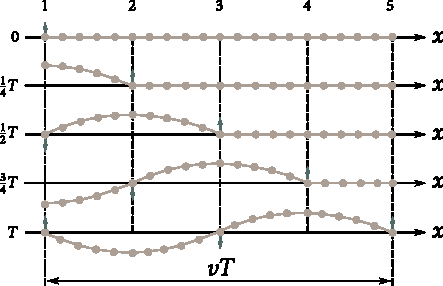
\includegraphics[scale=1]{figures/ch_14/fig_14_1.pdf}
		\caption[]{}
		\label{fig:14_1}
	\end{center}
	\vspace{-1mm}
\end{figure}

\begin{figure}[!htb]
	\begin{center}
		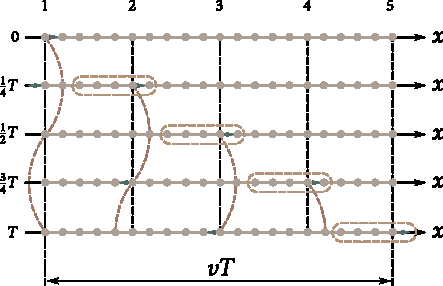
\includegraphics[scale=1]{figures/ch_14/fig_14_2.pdf}
		\caption[]{}
		\label{fig:14_2}
	\end{center}
\end{figure}

Hình \ref{fig:14_2} cho thấy các hạt chuyển động như thế nào khi một sóng dọc truyền trong một môi trường. Tất cả các lý luận liên quan đến hành vi của các phần tử trong sóng ngang cũng tương tự trường hợp sóng dọc với các chuyển động sang phải sang trái được thay thế cho các chuyển động lên xuống. Nhìn qua hình cho thấy sự lan truyền của sóng dọc trong một môi trường có sự bù trừ và giãn nở xen kẽ của các phần tử (vị trí bù của các phần tử được bao quanh bởi một đường gạch ngang trong hình). Chúng chuyển động theo phương truyền sóng với vận tốc $v$.

Hình \ref{fig:14_1} và hình \ref{fig:14_2} biểu diễn dao động của các hạt có vị trí cân bằng nằm trên trục $x$. Trên thực tế, không chỉ các phần tử dọc theo trục $x$, mà toàn bộ tập hợp các phần tử có trong một thể tích nhất định đều dao động. Lan truyền từ nguồn dao động, quá trình sóng liên quan đến các phần mới và mới của không gian. Quỹ tích của các điểm vừa bắt đầu dao động tại thời điểm $t$ được gọi là \textbf{mặt đầu sóng}. Mặt sau là bề mặt ngăn cách phần không gian đã tham gia vào quá trình sóng với vùng chưa xuất hiện dao động.

\begin{figure}[!htb]
	\begin{center}
		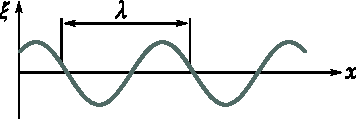
\includegraphics[scale=1]{figures/ch_14/fig_14_3.pdf}
		\caption[]{}
		\label{fig:14_3}
	\end{center}
	\vspace{-0.85cm}
\end{figure}

Quỹ tích các điển dao động đồng pha được gọi là \textbf{mặt sóng}. Một bề mặt sóng có thể được vẽ qua bất kỳ điểm nào trong không gian tham gia vào quá trình dao động của sóng. Vì vậy, có vô số mặt sóng nhưng lại chỉ có một đầu sóng tại mỗi thời điểm. Các mặt sóng luôn duy trì trạng thái đứng yên (chúng chỉ qua lại vị trí cân bằng của các phần tử dao động cùng pha). Còn một mặt đầu sóng luôn chuyển động.

Mặt sóng có thể có hình dạng bất kì. Ví dụ đơn giản, chúng có thể là mặt phẳng hoặc mặt cầu. Sóng trong trường hợp này được gọi là \textbf{sóng phẳng} và \textbf{sóng cầu}. Trong sóng phẳng, các mặt sóng là vô số các mặt phẳng song song với nhau, trong sóng cầu thì các mặt sóng là vô số các mặt cầu đồng tâm.

Giả sử có một sóng phẳng truyền theo trục $x$. Tất cả các điểm trong môi trường có vị trí cân bằng xác định bởi toạ độ $x$ (nhưng có các toạ độ $y$ và $z$ khác nhau) sẽ dao động cùng pha. Hình \ref{fig:14_3} biểu diễn đường cong tạo bởi li độ $\xi$ của các điểm có toạ độ $x$ khác nhau tại một thời điểm xác định. Hình vẽ này không được hiểu là hình ảnh của một sóng. Nó chỉ đưa ra một đồ thị của hàm $\xi(x,t)$ tại một thời điểm xác định. Đồ thị này có thể tạo nên bởi cả sóng dọc và sóng ngang. 

Khoảng cách $\lambda$ mà sóng truyền được trong một chu kỳ dao động của các phần tử trong môi trường được gọi là \textbf{bước sóng}. Rõ ràng rằng
\begin{equation}\label{eq:14_1}
    \lambda = vT,
\end{equation}

\noindent
với $v$ là vận tốc truyền sóng \\
\indent $T$ là chu kỳ dao động.

Bước sóng cũng có thể được định nghĩa là khoảng cách giữa 2 phần tử gần nhât của môi trường có độ lệch pha bằng $2\pi$ (xem \fig{14_3}).

Thay $1/\nu$ ($\nu$ là tần số của các dao động) cho $T$ trong \eqn{14_1}, ta được
\begin{equation}\label{eq:14_2}
    \lambda\nu = v.
\end{equation}

\noindent
Ta có thể dẫn ra được biểu thức này bằng cách lâp luận sau. Trong mỗi giây, một nguồn sóng hoàn thành được $\nu$ dao động, tạo ra một lần ``nhấp'' và một lần ``nhô'' trong quá trình dao động. Tại thời điểm nguồn hoàn thành $\nu$ dao động, lần nhô đầu tiên đã đi được một khoảng $v$. Do đó, trên đoạn đường $v$ phải gồm $\nu$ đỉnh nhấp và nhô của sóng.

\section{Phương trình của sóng phẳng và sóng cầu}\label{sec:14_2}

Một phương trình sóng là sự biểu diễn ly độ của một dao phần tử đang dao động như một hàm của toạ độ $x$, $y$, $z$ của nó và thời gian $t$:
\begin{equation}\label{eq:14_3}
    \xi = \xi(x,y,z,t)
\end{equation}

\noindent
(Ta hiểu trong đầu rằng toạ độ ở đây chỉ vị trí cân bằng của các phần tử). Hàm sóng này phải là hàm tuần hoàn theo cả thời gian $t$ và theo các toạ độ $x$, $y$, $z$. Tính tuần hoàn của nó theo thời gian dựa trên viêc $\xi$ mô tả dao động của một hạt có tọa độ $x$, $y$, $z$. Tính tuần hoàn của nó đối với các tọa độ dựa trên việc các điểm cách nhau một khoảng $\lambda$ sẽ dao động y như nhau.

Ở đây ta sẽ khảo sát hàm $\xi$ cho sóng phẳng dao động điều hoà. Để đơn giản, ta sẽ chọn trục $x$ của hệ toạ độ trùng với phương truyền sóng. Mặt sóng vì vậy sẽ vuông góc với trục $x$ và bởi vì tất cả các điểm trên mặt sóng dao động như nhau nên li độ $\xi$ sẽ chỉ phụ thuộc vào $x$ và $t$, tức là $\xi=\xi(x,t)$. Dao động của một điểm tại mặt phẳng $x=0$ (\fig{14_4}) sẽ có dạng
\begin{equation*}
    \xi(0,t) = A \cos(\omega t + \alpha).
\end{equation*}

\begin{figure}[!htb]
	\begin{center}
		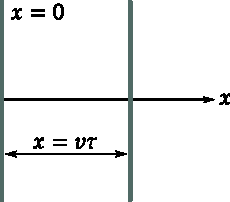
\includegraphics[scale=1]{figures/ch_14/fig_14_4.pdf}
		\caption[]{}
		\label{fig:14_4}
	\end{center}
	\vspace{-0.85cm}
\end{figure}

\noindent
Giờ ta sẽ tìm dạng dao động của một điểm trên mặt phẳng ứng với một giá trị $x$ tùy ý. Để đi được quãng đường từ mặt phẳng $x=0$ đến mặt phẳng này, sóng cần thời gian $T=x/v$ (ở đây, $v$ là vận tốc truyền sóng). Do đó, dao động của các hạt trong mặt phẳng $x$ sẽ trễ hơn một thời gian $T$ so với dao động của các hạt trong mặt phẳng $x=0$, tức là chúng sẽ có dạng
\begin{equation*}
    \xi(x,t) = A \cos[\omega(t - \tau) + \alpha] = A \cos\bracket{ \omega \parenthesis{t - \frac{x}{v}} + \alpha}.
\end{equation*}

Do đó, phương trình của sóng phẳng (cả sóng dọc và sóng ngang) truyền theo phương của trục $x$ có dạng sau:
\begin{equation}\label{eq:14_4}
    \xi = A \cos\bracket{ \omega \parenthesis{t - \frac{x}{v}} + \alpha}.
\end{equation}

\noindent
Đại lượng $A$ là biên độ của sóng.
Pha ban đầu của sóng $\alpha$ được xác định bởi sự lựa chọn của chúng ta về điểm bắt đầu khảo sát $x$ và $t$.
Khi khảo sát một sóng, thời điểm ban đầu và tọa độ thường được chọn sao cho $\alpha=0$.
Việc chọn này sẽ không thể thực hiện được khi khảo sát đồng thời nhiều sóng.

Giờ ta sẽ gán một giá trị cho pha trong biểu thức \eqn{14_4} bởi giả thiết
\begin{equation}\label{eq:14_5}
    \omega \parenthesis{t - \frac{x}{v}} + \alpha = \text{constant}.
\end{equation}

\noindent
Biểu thức này xác định mối quan hệ giữa thời gian $t$ và nơi $x$ mà pha có giá trị cố định. Giá trị của $\diffin{x}{t}$ cho biết vận tốc của pha truyền đi. Đạo hàm biểu thức \eqn{14_5} ta được
\begin{equation*}
    \deriv{t} - \frac{1}{v}\, \deriv{x} = 0,
\end{equation*}

\noindent
từ đó
\begin{equation}\label{eq:14_6}
    \diff{x}{t} = v.
\end{equation}

\noindent
Vì vậy, vận tốc truyền của sóng $v$ trong \eqn{14_4} là vận tốc truyền pha, và trong liên hệ này thì được gọi là \textbf{vận tốc pha}.

Từ biểu thức \eqn{14_6}, ta có $\diffin{x}{t}>0$. Vì vậy, \eqn{14_4} mô tả một sóng truyền theo chiều dương của trục $x$. Một sóng truyền theo chiều ngược lại sẽ được mô tả bởi phương trình
\begin{equation}\label{eq:14_7}
    \xi = A \cos\bracket{ \omega \parenthesis{t + \frac{x}{v}} + \alpha}.
\end{equation}

\noindent
Thật vậy, cân bằng pha của sóng \eqref{eq:14_7} với một hằng số và đạo hàm phương trình vừa thu được, chúng ta dẫn ra biểu thức
\begin{equation*}
    \diff{x}{t} = -v,
\end{equation*}

\noindent
điều đó cho thấy sóng cho bởi phương trình \eqn{14_7} truyền theo chiều giảm dần của trục $x$.

Phương trình của sóng phẳng có thể cho bởi sự mối quan hệ đối xứng giữa $x$ và $t$. Để thấy được điều đó, ta sẽ đưa ra một đại lượng
\begin{equation}\label{eq:14_8}
    k = \frac{2\pi}{\lambda},
\end{equation}

\noindent
được hiểu là \textbf{số sóng}. Nhân cả tử số và mẫu số vế phải của biểu thức \eqn{14_8} với tần số $\nu$, ta có thể biểu diễn số sóng dưới dạng
\begin{equation}\label{eq:14_9}
    k = \frac{\omega}{\nu}
\end{equation}

\noindent
[xem \eqn{14_2}]. Thay \eqn{14_9} vào trong ngoặc của biểu thức \eqn{14_4}, ta đưa đến phương trình cho một sóng phẳng truyền theo trục $x$:
\begin{equation}\label{eq:14_10}
    \xi = A \cos(\omega t - kx + \alpha).
\end{equation}

\noindent
Phương trình truyền sóng theo chiều giảm của $x$ sẽ chỉ khác so với \eqn{14_10} về dấu của thành phần $kx$.

Để dẫn ra biểu thức \eqn{14_10}, ta đã giả sử rằng biên độ của dao động không hề phụ thuộc vào $x$. Điều này khá hiển nhiên với sóng phẳng khi mà năng lượng của sóng không bị hấp thụ bởi môi trường. Nhưng khi sóng truyền qua môi trường có sự hấp thụ năng lượng, cường độ của sóng giảm dần theo khoảng cách từ nguồn dao động---sự tắt dần của sóng là điều có thể thấy được. Thực nghiệm cho thấy trong các môi trường đồng nhất thì sự tắt dần của các sóng tuân theo quy luật: $A = A_0 e^{-\gamma x}$ [tương tự với sự giảm dần biên độ theo thời gian; xem Eq. (7.102) of Vol. I]. Theo đó, phương trình của sóng phẳng sẽ có dạng:
\begin{equation}\label{eq:14_11}
    \xi = A_0\, e^{-\gamma x} \cos(\omega t - kx + \alpha)
\end{equation}

\noindent
($A_0$ là biên độ tại mặt phẳng $x=0$, và $\gamma$ là hệ số suy hao).

Giờ ta sẽ tìm phương trình tương tự với sóng cầu. Bất kỳ nguồn sóng thực nào cũng có một độ phân tán nhất định. Nhưng nếu ta tự giới hạn khảo sát một sóng ở khoảng cách đủ lớn so với kích thước của nguồn, ta có thể tạm coi sóng như một chất điểm. Sóng phát ra từ một điểm trong một môi trường đồng nhất và đẳng hướng sẽ có dạng hình cầu. Giả sử rằng pha dao động của nguôn là $(\omega t + \alpha)$. Do đó các điểm trên mặt sóng bán kính $r$ sẽ dao động với pha $\omega (t - r/v) + \alpha = \omega_0t - kr + \alpha$ (sóng cần thời gian $\tau = r/v$ để đi được đoạn $r$). Ngay cả khi xem rằng môi trường truyền sóng không hấp thụ năng lượng, biên đô dao động trong trường hợp này vẫn không được giữ nguyên---nó vẫn giảm theo khoảng cách từ nguồn theo hàm $1/r$ (xem \sect{14_6}). Do đó phương trình sóng cầu sẽ có dạng
\begin{equation}\label{eq:14_12}
    \xi = \frac{A}{r} \cos(\omega t - kr + \alpha),
\end{equation}

\noindent
trong đó $A$ là một đại lượng không đổi bằng số bằng biên độ tại một khoảng cách xác định từ nguồn. Thứ nguyên của $A$ bằng thứ nguyên của đại lượng dao động nhân với thứ nguyên của độ dài. Hệ số $e^{-\gamma r}$ phải được nhân với biểu thức \eqn{14_12} với trường hợp môi trường có sự hấp thụ.

Ta nhắc lại với độc giả rằng các giả thiết của chúng ta, \eqn{14_12} chỉ dùng được với $r$ đủ lớn so với kích thước của nguồn. Khi $r$ tiến đến $0$, hàm biểu diễn biên độ sẽ tiến đến vô cùng. Để giải thích cho kết quả bất thường này, có thể nói phương trình trên không thể sử dụng với giá trị $r$ nhỏ.

\section{Phương trình sóng phẳng truyền theo phương bất kì}\label{sec:14_3}

Ở phần này, ta sẽ tìm biểu thức của một sóng phẳng lan truyền theo hướng tạo với góc $\alpha$, $\beta$, $\gamma$ (không tính đến hệ số suy hao) với các trục toạ độ $x$, $y$, $z$. Ta sẽ giả thiết rằng các dao động trong mặt phẳng đi qua gốc toạ độ (\fig{14_5}) có dạng
\begin{equation}\label{eq:14_13}
    \xi_0 = A \cos(\omega t + \alpha).
\end{equation}

\begin{figure}[!htb]
	\begin{center}
		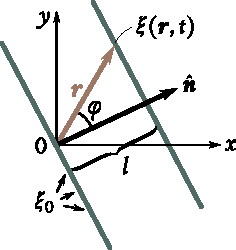
\includegraphics[scale=1]{figures/ch_14/fig_14_5.pdf}
		\caption[]{}
		\label{fig:14_5}
	\end{center}
	\vspace{-0.8cm}
\end{figure}

\noindent
Ta đặt mặt sóng (phẳng) ở khoảng cách $l$ từ gốc toạ độ. Dao động trong mặt phẳng sẽ bị chậm so với các dao động được mô tả bởi \eqn{14_13} một khoảng thời gian $\tau=l/v$:
\begin{equation}\label{eq:14_14}
    \xi = A \cos\bracket{ \omega \parenthesis{t - \frac{l}{v}} + \alpha} = A \cos(\omega t - kl + \alpha)
\end{equation}

\noindent
[$k = \omega/v$; xem \eqn{14_9}].

Ta biểu diễn $l$ theo các toạ độ vector của các điểm trên mặt sóng mà ta đang khảo sát. Để làm vậy, ta sẽ đưa ra một vector đơn vị $\hatvec{n}$ của pháp tuyến của mặt sóng. Hình \fig{14_5} cho thấy tích vô hướng của $\hatvec{n}$ và toạ độ vector của $\vec{r}$ của mỗi điểm trên mặt phẳng là $l$:
\begin{equation*}
    \hatvec{n} \ccdot \vec{r} = r\cos\varphi = l.
\end{equation*}

\noindent

Thay $\hatvec{n}\ccdot\vec{r}$ cho $l$ trong \eqn{14_14} ta được
\begin{equation}\label{eq:14_15}
    \xi = A \cos[\omega t - k (\hatvec{n}\ccdot\vec{r}) + \alpha].
\end{equation}

Vector
\begin{equation}\label{eq:14_16}
    \vec{k} = k \hatvec{n},
\end{equation}

\noindent
có độ lớn bằng số sóng $k=2\pi/\lambda$ và hướng dọc theo hướng pháp tuyến của mặt sóng được gọi là \textbf{vector sóng}. Từ đó, \eqn{14_15} có thể được viết dưới dạng
\begin{equation}\label{eq:14_17}
    \xi(\vec{r},t) = A \cos(\omega t - \vec{k} \ccdot \vec{r} + \alpha).
\end{equation}

\noindent
Ta thu được biểu thức cho một sóng phẳng không suy hao truyền theo một hướng xác định bởi vector sóng $\vec{k}$. Với một sóng có suy hao, ta phải thêm vào biểu thức một hệ số  $e^{-\gamma l}=e^{-\gamma (\hatvec{n}\ccdot\vec{r})}$.

Biểu thức \eqref{eq:14_17} cho biết độ lệch của một điểm có vector vị trí $\vec{r}$ so với vị trí cân bằng của nó tại thời điểm $t$ (ta nhấn mạnh với người đọc rằng $\vec{r}$ xác định vị trí cân bằng của chất điểm). Để chuyển từ vectơ vị trí của một điểm đến tọa độ $x$, $y$, $z$ của nó, ta biểu diễn tích vô hướng $\vec{k} \ccdot \vec{r}$ thông qua các thành phần của vector dọc theo trục tọa độ:
\begin{equation*}
    \vec{k}\ccdot\vec{r} = k_x x + k_y y + k_z z.
\end{equation*}

\noindent
Từ đó, biểu thức của một sóng phẳng trở thành
\begin{equation}\label{eq:14_18}
    \xi(x,y,z; t) = A \cos\parenthesis{ \omega t - k_x x - k_y y - k_z z + \alpha}.
\end{equation}

\noindent
Vì vậy,
\begin{equation}\label{eq:14_19}
    k_x = \frac{2\pi}{\lambda}\cos\alpha,\quad k_y = \frac{2\pi}{\lambda}\cos\beta, \quad k_z = \frac{2\pi}{\lambda}\cos\gamma.
\end{equation}

\noindent
Biểu thức \eqref{eq:14_18} cho biết độ lệch của một điểm có toạ độ $x$, $y$, $z$ tại thời điểm $t$. Khi $\hatvec{n}$ song song với $\vecuni{x}$, ta có $k_x = x$, $k_y = k_z = 0$, và \eqn{14_18} trở thành \eqn{14_10}. Sẽ vô cùng thuận tiện khi ta viết lại biểu thức của sóng phẳng dưới dạng
\begin{equation}\label{eq:14_20}
    \xi = \Re\bracket{ A e^{i(\omega t - \vec{k}\ccdot\vec{r} + \alpha)} }.
\end{equation}

\noindent
Ký hiệu $\Re$ thường được bỏ qua, nhưng hãy nhớ trong đầu rằng ta chỉ lấy phần thực của nó. Dựa vào đó, số phức
\begin{equation}\label{eq:14_21}
    \hat{A} = A e^{i\alpha},
\end{equation}

\noindent
được gọi là \textbf{biên độ phức} được đưa ra. Trị tuyệt đối của số phức này chính là biên độ, và argument của nó chính là pha ban đầu của sóng.

Như vậy, biểu thức của sóng phẳng không suy hao có thể được viết dưới dạng
\begin{equation}\label{eq:14_22}
    \xi = \hat{A} e^{i(\omega t - \vec{k}\ccdot\vec{r})}.
\end{equation}

\noindent
Lợi ích của cách viết này sẽ được thấy trong các phần sau.

\section{Phương trình sóng}\label{sec:14_4}

Biểu thức của một sóng bất kỳ là nghiệm của phương trình vi phân được gọi là \textbf{phương trình sóng}. Để thành lập dạng của phương trình sóng, ta so sánh các đạo hàm cấp 2 theo toạ độ và thời gian của biểu thức mô tả một sóng phẳng \eqref{eq:14_18}. Lấy đạo hàm riêng phần 2 lần theo từng biến, ta được
\begin{align*}
    \diffnpartial{\xi}{t}{2} = -\omega^2 A \cos(\omega t - \vecdot{k}{r} + \alpha) = -\omega^2 \xi,\\
    \diffnpartial{\xi}{x}{2} = -k_x^2 A \cos(\omega t - \vecdot{k}{r} + \alpha) = -k_x^2 \xi,\\
    \diffnpartial{\xi}{y}{2} = -k_y^2 A \cos(\omega t - \vecdot{k}{r} + \alpha) = -k_y^2 \xi,\\
    \diffnpartial{\xi}{t}{2} = -k_z^2 A \cos(\omega t - \vecdot{k}{r} + \alpha) = -k_z^2 \xi.
\end{align*}

\noindent
Lấy tổng các đạo hàm riêng phần theo toạ độ, ta được
\begin{equation}\label{eq:14_23}
    \diffnpartial{\xi}{x}{2} + \diffnpartial{\xi}{y}{2} + \diffnpartial{\xi}{z}{2} = - (k_x^2 + k_y^2 + k_z^2) \xi = -k^2 \xi.
\end{equation}

\noindent
So sánh tổng này với đạo hàm riêng phần theo thời gian và thay $1/v^2$ cho $k^2/\omega^2$ [xem \eqn{14_9}], ta được biểu thức
\begin{equation}\label{eq:14_24}
    \diffnpartial{\xi}{x}{2} + \diffnpartial{\xi}{y}{2} + \diffnpartial{\xi}{z}{2} = \frac{1}{v^2}\, \diffnpartial{\xi}{t}{2}.
\end{equation}

\noindent
Đây chính xác là phương trình sóng. Nó còn có thể viết dưới dạng
\begin{equation}\label{eq:14:25}
    \upDelta{\xi} = \frac{1}{v^2}\, \diffnpartial{\xi}{t}{2},
\end{equation}

\noindent
với $\upDelta$ là toán tử Laplace [xem \eqn{1_104}].

Khá dễ dàng để thấy rằng không chỉ có hàm sóng thảo mãn \eqref{eq:14_18} mà còn cả bất cứ hàm nào có dạng
\begin{equation}\label{eq:14_26}
    f(x,y,z;t) = f(\omega t - k_x x - k_y y - k_z z + \alpha).
\end{equation}

\noindent
Thật vậy, biểu thị biểu thức trong ngoặc đơn ở phía bên phải của \eqn{14_26} bằng hàm $\zeta$, ta có
\begin{equation}\label{eq:14_27}
    \diffpartial{\zeta}{t} = \diffpartial{f}{\zeta} \diffpartial{\zeta}{t} = f' \omega,\quad \diffnpartial{f}{t}{2} = \omega \diffpartial{f'}{\zeta} \diffpartial{\zeta}{t} = \omega^2 f''.
\end{equation}

\noindent
Tương tự,
\begin{equation}\label{eq:14_28}
    \diffnpartial{f}{x}{2} = k_x^2 f'',\quad \diffnpartial{f}{y}{2} = k_y^2 f'',\quad \diffnpartial{f}{z}{2} = k_z^2 f''.
\end{equation}

\noindent
Đưa \eqns{14_27}{14_28} vào \eqn{14_24}, ta đưa đến kết luận rằng hàm \eqref{eq:14_26} thoả mãn phương trình sóng nếu ta xem rằng $v = \omega/k$.

Bất kỳ hàm nào thoả mãn phương trình có dạng \eqn{14_24} đều mô tả một sóng; căn bậc 2 của nghịch đảo hệ số của $\diffnpartialin{\xi}{t}{2}$ chính là vận tốc pha của sóng này.

Chúng ta phải lưu ý rằng đối với một sóng phẳng truyền dọc theo trục $x$, phương trình sóng có dạng
\begin{equation}\label{eq:14_29}
    \diffnpartial{\xi}{x}{2} = \frac{1}{v^2} \diffnpartial{\xi}{t}{2}.
\end{equation}

\section{Vận tốc sóng đàn hồi trong chất rắn}\label{sec:14_5}

\begin{figure}[!htb]
	\begin{center}
		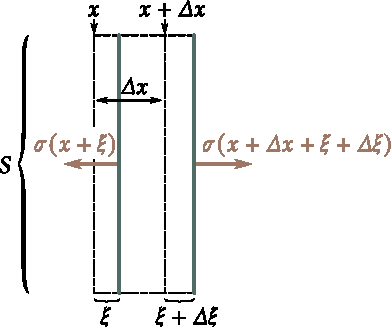
\includegraphics[scale=1]{figures/ch_14/fig_14_6.pdf}
		\caption[]{}
		\label{fig:14_6}
	\end{center}
	\vspace{-0.8cm}
\end{figure}

Giả sử rằng có một sóng dọc truyền theo trục $x$. Ta chia thể tích môi trường hình trụ thành những hình trụ có diện tích đáy $S$ và độ cao $\Delta{x}$ (\fig{14_6}). Li độ $\xi$ của các phần tử vị trí $x$ khác nhau sẽ khác nhau tại mỗi thời điểm (xem \fig{14_6} cho thấy $\xi$ so với $x$). Nếu đáy hình trụ toạ độ $x$ có li độ $\xi$ tại một thời điểm xác định, li độ của đáy toạ độ $x+\Delta{x}$ sẽ là $\xi+\Delta{\xi}$. Từ đó, thể tích đang được xét sẽ bị kéo dài thêm $\Delta{\xi}$ ($\Delta{\xi}$ là giá trị đại số, $\Delta{\xi}<0$ là trường hợp hình trụ bị nén lại) hay độ giãn dài tương đối là $\Delta{\xi}/\Delta{x}$. Đại lượng $\Delta{\xi}/\Delta{x}$ biểu diễn độ biến dạng trung bình của hình trụ. Vì $\xi$ biến thiên theo $x$ với quy luật không tuyến tính, độ biến dạng thực của một mặt cắt hình trụ khác nhau sẽ có giá trị khác nhau. Để xác định độ biến dạng của mặt cắt $x$, ta phải lấy $\Delta{x}$ tiến đến không. Như vậy,
\begin{equation}\label{eq:14_30}
	\varepsilon = \diffpartial{\xi}{x}
\end{equation}

\noindent
(Ta dùng ký hiệu vi phân riêng phần vì $\xi$ không chỉ phụ thuộc vào $x$ mà còn phụ thuộc cả vào $t$).

Sự xuất hiện của biến dạng kéo cho thấy tồn tại một ứng suất pháp tuyến $\sigma$ cho biến dạng nhỏ tỷ lệ với độ biến dạng. Theo phương trình (2.30) của Tập I,
\begin{equation}\label{eq:14_31}
	\sigma = E \varepsilon = E = \diffpartial{\xi}{x}
\end{equation}

\noindent
($E$ là suất Young của môi trường). Ta cần lưu ý rằng biến dạng thành phần và cả ứng suất $\sigma$ đều phụ thuộc vào $x$ tại một thời điểm xác định (\fig{14_7}). Khi độ lệch của các phần từ tới vị trí cân bằng của chúng đạt cực đại, sự kéo và dãn đều bằng không. Khi các phần tử đi qua vị trí cân bằng của chúng, sự kéo và nén tiến tới giá trị cực đại, các giá trị âm và dương của lực căng (tức là sức căng và sức nén) thay đổi luân phiền. Theo đó, ta đã ghi chú ở \sect{14_1}, một sóng dọc bao gồm các sự nén dãn luân phiên của môi trường.

\begin{figure}[!htb]
	\begin{center}
		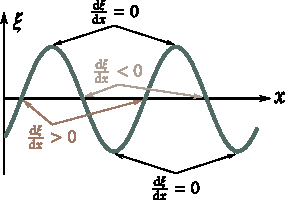
\includegraphics[scale=1.1]{figures/ch_14/fig_14_7.pdf}
		\caption[]{}
		\label{fig:14_7}
	\end{center}
	\vspace{-0.8cm}
\end{figure}

Ta quay lại với phần hình trụ được mô tả ở \fig{14_6} và viết phương trình chuyển động cho nó. Giả thiết rằng $\Delta{x}$ rất nhỏ, ta có thể xét hình chiếu của gia tốc lên trục $x$ giống như tất cả các điểm của hình trụ đó và bằng $\diffnpartialin{\xi}{t}{2}$. Khối lượng của hình trụ là $\rho S\Delta{x}$, với $\rho$ là khối lượng riêng của môi trường khi xem như biến dạng không đáng kể. Hình chiếu theo trục $x$ của lực tác dụng lên hình trụ bằng tích của diện tích $S$ của đáy hình trụ và hiệu của 2 ứng suất pháp tuyến của các mặt cắt $(x+\Delta{x} +\xi + \Delta{\xi})$ và $(x+\xi)$:
\begin{equation}\label{eq:14_32}
	F_x = SE \bracket{ \parenthesis{ \diffpartial{\xi}{x} }_{x + \Delta{x} +\xi + \Delta{\xi}} - \parenthesis{ \diffpartial{\xi}{x} }_{x + \xi} }.
\end{equation}

Giá trị của đạo hàm $\diffpartialin{\xi}{x}$ tại mặt cắt $x + \delta$ có thể được viết với một độ sấp sỉ tốt cho giá trị nhỏ của $\delta$ có dạng
\begin{equation}\label{eq:14_33}
	\parenthesis{ \diffpartial{\xi}{x} }_{x+\delta} = \parenthesis{ \diffpartial{\xi}{x} }_{x} + \bracket{ \diffpartial{}{x} \parenthesis{ \diffpartial{\xi}{x} } }_x\, \delta = \parenthesis{ \diffpartial{\xi}{x} }_{x} + \diffnpartial{\xi}{x}{2}\, \delta,
\end{equation}

\noindent
với $\diffnpartialin{\xi}{x}{2}$ là đạo hàm riêng phần cấp 2 của $\xi$ theo $x$ tại mặt cắt $x$.

Do các đại lượng $\Delta{x}$, $\xi$, và $\Delta{\xi}$ vô cùng nhỏ, ta có đưa \eqref{eq:14_33} vào \eqn{14_32}:
\begin{align}
	F_x &= SE \bracet{
	\bracket{
	\parenthesis{ \diffpartial{\xi}{x} }_{x}  + \diffnpartial{\xi}{x}{2} (\Delta{x}+\xi+\Delta{\xi})
	} -
	\bracket{
	\parenthesis{ \diffpartial{\xi}{x} }_{x} + \diffnpartial{\xi}{x}{2} \xi
	}
	}\nonumber\\
	&= SE \diffnpartial{\xi}{x}{2} (\Delta{x} + \Delta{\xi}) \approx SE \diffnpartial{\xi}{x}{2} \Delta{x} \label{eq:14_34}
\end{align}

\noindent
[Độ dãn dài tương đối $\diffpartialin{\xi}{x}$ trong biến dạng đàn hồi nhỏ hơn rất nhiều một đơn vị. Thật vậy, $\Delta{\xi}\ll\Delta{x}$ nên sự bổ sung $\Delta{\xi}$ trong tổng $(\Delta{x} + \Delta{\xi})$ có thể bỏ qua].

Thay các giá trị tìm được của khối lượng, gia tốc và lực vào phương trình định luật II Newton, ta được
\begin{equation*}
	\rho S \Delta{x} \diffnpartial{\xi}{t}{2} = SE \diffnpartial{\xi}{x}{2} \Delta{x}.
\end{equation*}

\noindent
Cuối cùng, khử $S\Delta{x}$, ta được phương trình
\begin{equation}\label{eq:14_35}
	\diffnpartial{\xi}{x}{2} = \frac{\rho}{E} \diffnpartial{\xi}{t}{2},
\end{equation}

\noindent
là phương trình sóng trong trường hợp $\xi$ không phụ thuộc vào $y$ và $z$. 
So sánh \eqns{14_29}{14_35} cho thấy
\begin{equation}\label{eq:14_36}
	v = \parenthesis{\frac{E}{\rho}}^{1/2},
\end{equation}

\noindent
Thật vậy, vận tốc pha của sóng đàn hồi dọc bằng căn bậc hai của tỷ số suất Young chia cho khối lượng riêng của môi trường.

Tính toán tương tự với sóng ngang cho ta biểu thức
\begin{equation}\label{eq:14_37}
	v = \parenthesis{\frac{G}{\rho}}^{1/2},
\end{equation}

\noindent
với $G$ là module cắt.

\section{Năng lượng của sóng đàn hồi}\label{sec:14_6}

Giả sử có một sóng dọc phẳng,
\begin{equation*}
	\xi = A \cos(\omega t - kx + \alpha)
\end{equation*}

\noindent
[xem \eqn{14_10}], đang truyền theo trục $x$ trong một môi trường xác định. Ta chia môi trường này thành các thể tích nguyên tố $\Delta{V}$ rất nhỏ sao cho vận tốc và sức căng tại mọi điểm trong thể tích này có thể xem là như nhau và lần lượt là $\diffpartialin{\xi}{t}$ và $\diffpartialin{\xi}{x}$.

Phần thể tích ta đã chia có động năng
\begin{equation}\label{eq:14_38}
	\ab{\Delta{W}}{k} = \frac{\rho}{2} \parenthesis{\diffpartial{\xi}{t}}^2 \Delta{V}
\end{equation}

\noindent
($\rho\Delta{V}$ là khối lượng của phần thể tích, và $\diffpartialin{\xi}{t}$ là vận tốc của nó).

Từ Eq. (3.81) of Vol. I, phần thể tích đang được xét có thế ngăng đàn hồi
\begin{equation*}
	\ab{\Delta{W}}{p} = \frac{E\varepsilon^2}{2} \Delta{V}  = \frac{E}{2} \parenthesis{\diffpartial{\xi}{x}}^2 \Delta{V}
\end{equation*}

\noindent
($\varepsilon=\diffpartialin{\xi}{x}$ là độ nén dài tỷ đối của hình trụ, $E$ là suất Young của môi trường). Ta đưa \eqn{14_36} để thay $\rho v^2$ cho suất Young ($\rho$ là khối lượng riêng của môi trường, và $v$ là phận tốc pha của sóng). Như vậy, biểu thức cho thế năng của khối lượng $\Delta{V}$ có dạng
\begin{equation}\label{eq:14_39}
	\ab{\Delta{W}}{p} = \frac{E\varepsilon^2}{2} \parenthesis{\diffpartial{\xi}{x}}^2 \Delta{V}.
\end{equation}

Tổng của \eqns{14_38}{14_39} chính là tổng năng lượng
\begin{equation}\label{eq:14_40}
	\Delta{W} = \ab{\Delta{W}}{k} + \ab{\Delta{W}}{p} = \frac{1}{2} \rho \bracket{ \parenthesis{\diffpartial{\xi}{t}}^2 + v^2 \parenthesis{\diffpartial{\xi}{x}}^2 } \Delta{V}.
\end{equation}

\noindent
Chia năng lượng này cho thể tích $\Delta{V}$, ta có mật độ năng lượng
\begin{equation}\label{eq:14_41}
	w = \frac{1}{2} \rho \bracket{ \parenthesis{\diffpartial{\xi}{t}}^2 + v^2 \parenthesis{\diffpartial{\xi}{x}}^2 }.
\end{equation}

Đạo hàm \eqn{14_10} một lần riêng phần theo $t$ và một lần riêng phần theo $x$ cho
\begin{align*}
	\diffpartial{\xi}{t} &= - A\omega \sin(\omega t - kx + \alpha),\\
	\diffpartial{\xi}{x} &=  kA \sin(\omega t - kx + \alpha).
\end{align*}

\noindent
Thay các biểu thức này vào \eqn{14_41} và tính $k^2v^2=\omega^2$, ta được
\begin{equation}\label{eq:14_42}
	w = \rho A^2 \omega^2 \sin^2(\omega t - kx + \alpha).
\end{equation}

\noindent
Tính toán tương tự cho mật độ năng lượng của sóng ngang.

Có thể thấy từ \eqn{14_42} đó là mật độ năng lượng tại mỗi thời điểm khác nhau tại mỗi điểm khác nhau trong không gian. Ở cùng một vị trí, mật độ năng lượng phụ thuộc theo thời gian theo hàm sin bình phương. Giá trị trung bình của hàm sin bình phương là một phần hai. Do đó, giá trị trung bình theo thời gian của mật độ năng lượng tại mỗi điểm trong môi trường truyền là
\begin{equation}\label{eq:14_43}
	\average{w} = \frac{1}{2} \rho A^2 \omega^2.
\end{equation}

\noindent
Mật độ năng lượng cho bởi \eqn{14_42} và giá trị trung bình của nó [\eqn{14_43}] tỷ lệ với mật độ khối lượng của môi trường $\rho$, bình phương tần số góc $\omega$, và bình phương biên độ sóng $A$. Đây là một liên hệ không chỉ đúng cho sóng phẳng không suy hao mà còn là cho các sóng bất kì (sóng phẳng có suy hao, sóng cầu,...)

Thật vật, một môi trường mà sóng truyền qua có một lượng năng lượng bổ sung. Sóng đi sau được cung cấp cho các phần tử khác nhau của môi trường từ nguồn dao động bởi chính nó; cho nên một sóng mang theo năng lượng với nó.
% Thus, a medium in which a wave is propagating has an additional store of energy. 
Năng lườn được truyền bởi sóng qua một bề mặt trong một đơn vị thời gian được gọi là \textbf{năng thông} truyền qua bề mặt này. Nếu năng lượng $\deriv{w}$ được truyền qua một bề mặt xác định trong thời gian $\deriv{t}$, thì năng thông $\Phi$ là
\begin{equation}\label{eq:14_44}
	\Phi = \diff{W}{t}.
\end{equation}

\noindent
Năng thông là một đại lượng vô hướng mà thứ nguyên bằng thứ nguyên năng lượng chia cho thứ nguyên thời gian, tức là trùng hợp cùng thứ nguyên với công suất. Vì vậy, $\Phi$ được đo bằng watts, \si{\erg\per\second} và các đơn vị tương tự.
% The energy flux is a scalar quantity whose dimension equals that of energy divided by the dimension of time, \ie, coincides with the dimension of power.
% Accordingly, $\Phi$ is measured in watts, \si{\erg\per\second}, etc.

Thông lượng năng lượng tại mỗi điểm khác nhau của môi trường có thể có độ lớn khác nhau. Để đặc trưng cho một dòng năng lượng tại mỗi điểm trong không gian, một đại lượng vector được gọi là \textbf{mật độ năng thông}. Nó bằng năng thông truyền qua mỗi đơn vị diện tích vuông góc với phương truyền năng lượng tại một điểm. Hướng của vector mật độ năng thông trùng với phương truyền năng lượng.
% The energy flux at different points of a medium can have a different intensity.
% To characterize the flow of energy at different points of space, a vector quantity called the \textbf{density of the energy flux} is introduced.
% It numerically equals the energy flux through a unit area placed at the given point perpendicular to the direction in which the energy is being transferred.
% The direction of the vector of the energy flux density coincides with that of energy transfer.

Giả sử rằng năng lượng $\deriv{w}$ được truyền trong suốt thời gian $\deriv{t}$ qua diện tích $\Delta{S}_{\perp}$ vuông góc với phương truyền sóng. Vì vậy mật độ năng thông sẽ là
% Assume that the energy $\deriv{W}$ is transferred during the time $\deriv{t}$ through the area $\Delta{S}_{\perp}$ perpendicular to the direction of propagation of a wave.
% The energy flux density will therefore be
\begin{equation}\label{eq:14_45}
	j = \frac{\Delta{\Phi}}{\Delta{S}_{\perp}} = \frac{\Delta{W}}{\Delta{S}_{\perp} \Delta{t}}
\end{equation}

\begin{figure}[!htb]
	\begin{center}
		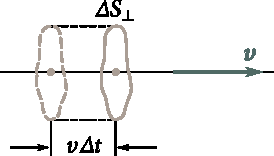
\includegraphics[scale=1]{figures/ch_14/fig_14_8.pdf}
		\caption[]{}
		\label{fig:14_8}
	\end{center}
	\vspace{-0.9cm}
\end{figure}

\noindent
[xem \eqn{14_44}].
Năng lượng $\Delta{W}$ của một hình trụ với mặt đáy $\Delta{S}_{\perp}$ và độ dài $v\Delta{t}$ ($v$ là vận tốc pha của sóng) sẽ truyền qua diện tích $\Delta{S}_{\perp}$ (\fig{14_8}) trong thời gian $\Delta{t}$. Nếu kích thước của hình trụ nhỏ (do $\Delta{S}_{\perp}$ và $\Delta{t}$ nhỏ) đủ để xem mật độ năng lượng tại mọi điểm trên hình trụ là đồng như nhau thì $\Delta{W}$ bằng tích của mật độ năng lượng $w$ và thể tích của hình trụ bằng $\Delta{S}_{\perp}v\Delta{t}$:
% The energy $\Delta{W}$ confined in a cylinder with the base $\Delta{S}_{\perp}$ and the altitude $v\Delta{t}$ ($v$ is the phase velocity of the wave) will be transferred through the area $\Delta{S}_{\perp}$ (\fig{14_8}) during the time $\Delta{t}$.
% If the dimensions of the cylinder are sufficiently small (as a result of the smallness of $\Delta{S}_{\perp}$ and $\Delta{t}$) to consider that the energy density at all points of the cylinder is the same, then $\Delta{W}$ can be found as the product of the energy density $w$ and the volume of the cylinder equal to $\Delta{S}_{\perp}v\Delta{t}$:
\begin{equation*}
	\Delta{W} = w \Delta{S}_{\perp} v \Delta{t}.
\end{equation*}

\noindent
Sử dụng biểu thức \eqn{14_45}, ta có phương trình cho mật độ năng lượng:
% Using this expression in \eqn{14_45}, we get the following equation for the density of the energy:
\begin{equation}\label{eq:14_46}
	j = wv.
\end{equation}

\noindent
Sau cùng, với vector $\vec{v}$ có độ lớn bằng vận tốc pha của sóng và hướng dọc theo phương truyền sóng (và truyền năng lượng), ta có thể viết
% Finally, introducing the vector $\vec{v}$ whose magnitude equals the phase velocity of the wave and whose direction coincides with that of wave propagation (and energy transfer), we can write
\begin{equation}\label{eq:14_47}
	\vec{j} = w \vec{v}.
\end{equation}

Ta biểu diễn được của vector mật độ năng thông. Vector này lần đầu tiên được đưa ra bởi nhà vật lý xuất chúng người Nga Nikolai Umov (1846-1915) và được gọi là \textbf{vector Umov}
% We have obtained an expression for the vector of the energy flux density.
% This vector was first introduced by the outstanding Russian physicist Nikolai Umov (1846-1915) and is called \textbf{Umov's vector}.

Vector được cho bởi \eqn{14_47} khác nhau tại mỗi điểm khác nhau trong không gian giống như mật độ năng lượng $w$. Ở mỗi điểm xác định, nó phụ thuộc vào thời gian theo hàm sin bình phương. Giá trị trung bình của nó là
% The vector given by \eqn{14_47}, like the energy density $w$, is different at different points of space.
% At a given point, it varies in time according to a sine square law.
% Its average value is
\begin{equation}\label{eq:14_48}
	\average{\vec{j}} = \average{w} \vec{v} = \frac{1}{2} \rho A^2 \omega^2 \vec{v}
\end{equation}

\noindent
[xem \eqn{14_43}].
Phương trình \eqref{eq:14_48}, giống như \eqn{14_43}, mô tả cho bất kỳ sóng nào (cầu, suy hao,...). Ta sẽ lưu ý rằng mỗi khi ta nói về cường độ của sóng tại mỗi điểm, ta sẽ hiểu là giá trị trung bình theo thời gian của mật độ năng thông truyền bởi sóng.
% We shall note that when we speak of the intensity of a wave at a given point, we have in mind the time-averaged value of the density of the energy flux transferred by the wave.

Khi biết $\vec{j}$ tại tất cả các điểm trên bề mặt $S$, ta có thể tính toán được năng thông truyền qua bề mặt này. Để làm vậy, ta sẽ chia bề mặt thành các diện tích nguyên tố $\deriv{S}$. Trong thời gian $\deriv{t}$, năng lượng $\deriv{w}$ chứa trong hình trụ xiên trong hình \fig{14_9} sẽ truyền qua diện tích $\deriv{S}$. Thể tích của hình trụ này là $\deriv{V} = v\, \deriv{t}\, \deriv{S}\, \cos\varphi$. Thể tích này chứa năng lượng $\deriv{W} = w\, \deriv{V} = wv\, \deriv{t}\, \deriv{S}\, \cos\varphi$ (ở đây, $w$ là giá trị đồng nhất của mật độ năng lượng tại diện tích $\deriv{S}$). Tính đến điều đó
% Knowing $\vec{j}$ for all the points of an arbitrary
% surface $S$, we can calculate the energy flux through this surface.
% For this purpose, let us divide the surface into elementary areas $\deriv{S}$.
% During the time $\deriv{t}$, the energy $\deriv{W}$ confined in the oblique cylinder shown in \fig{14_9} will pass through area $\deriv{S}$.
% The volume of this cylinder is $\deriv{V} = v\, \deriv{t}\, \deriv{S}\, \cos\varphi$.
% It contains the energy $\deriv{W} = w\, \deriv{V} = wv\, \deriv{t}\, \deriv{S}\, \cos\varphi$ (here, $w$ is the instantaneous value of the energy density where area $\deriv{S}$ is).
% Taking into account that
\begin{equation*}
	wv\, \deriv{S}\, \cos\varphi = j\, \deriv{S}\, \cos\varphi = \vec{j} \ccdot \derivec{S}
\end{equation*}

\noindent
($\derivec{S}=\hatvec{n}\,\deriv{S}$; xem \fig{14_9}), ta có thể viết: $\deriv{W} = \vec{j} \ccdot \derivec{S}\, \deriv{t}$. Từ đó, ta có được phương trình của năng thông $\deriv{\Phi}$ truyền qua diện tích $\deriv{S}$ như sau:
% ($\derivec{S}=\hatvec{n}\,\deriv{S}$; see \fig{14_9}), we can write: $\deriv{W} = \vec{j} \ccdot \derivec{S}\, \deriv{t}$.
% Hence, we obtain the following equation for the energy flux $\deriv{\Phi}$ through area $\deriv{S}$:
\begin{equation}\label{eq:14_49}
	\deriv{\Phi} = \diff{W}{t} = \vec{j} \ccdot \derivec{S}
\end{equation}

\begin{figure}[!htb]
	\begin{center}
		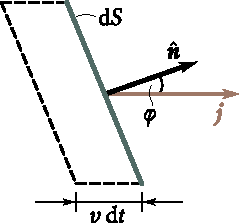
\includegraphics[scale=0.95]{figures/ch_14/fig_14_9.pdf}
		\caption[]{}
		\label{fig:14_9}
	\end{center}
	\vspace{-0.9cm}
\end{figure}

\noindent
[so sánh với \eqn{1_72}]. Tổng năng thông truyền qua một bề mặt bằng tổng các dòng nguyên tố cho bởi \eqn{14_49}:
% [compare with \eqn{1_72}].
% The total energy flux through a surface equals the sum of the elementary fluxes given by \eqn{14_49}:
\begin{equation}\label{eq:14_50}
	\Phi = \int_S \vec{j} \ccdot \derivec{S}.
\end{equation}

\noindent
Theo \eqn{1_74}, chúng ta có thể nói rằng năng thông bằng với thông lượng của vectơ $\vec{j}$ qua bề mặt $S$.

Thay cho vector $\vec{j}$ trong \eqn{14_50}, ta lấy giá trị trung bình theo thời gian của nó, ta có giá trị trung bình của $\Phi$:
% Substituting for the vector $\vec{j}$ in \eqn{14_50} its time-averaged value, we get the average value of $\Phi$:
\begin{equation}\label{eq:14_51}
	\average{\Phi} = \int_S \average{\vec{j}} \ccdot \derivec{S}.
\end{equation}

Ta sẽ tính giá trị của năng thông của một mặt sóng bất kỳ của một sóng cầu suy hao. Tại mỗi điểm trên bề mặt này, vector $\vec{j}$ cùng phương với $\derivec{S}$. Thêm vào đó, độ lớn của vector $\vec{j}$ cho mọi điểm trên một bề mặt là xác định. Vì vậy,
% Let us calculate the mean value of the energy flux through an arbitrary wave surface of an undamped spherical wave.
% At each point of this surface, the vectors $\vec{j}$ and $\derivec{S}$ coincide in direction.
% In addition, the magnitude of the vector $\vec{j}$ for all points of the surface is identical.
% Hence,
\begin{equation*}
	\average{\Phi} = \int_S \average{j}\, \deriv{S} = \average{j} S = \average{j} 4\pi r^2
\end{equation*}

\noindent
($r$ là bán kính của mặt sóng). Từ \eqn{14_48}, ta có $\average{j}=\rho A^2\omega^2v/2$. Vì thế,
% ($r$ is the radius of the wave surface).
% According to \eqn{14_48}, we have $\average{j}=\rho A^2\omega^2v/2$.
% Thus,
\begin{equation*}
	\average{\Phi} = 2\pi \rho \omega^2 A_r^2 r^2
\end{equation*}

\noindent
($A_r$ là biên độ sóng tại khoảng cách $r$ từ nguồn). Vì năng lượng của sóng không bị hấp thụ bởi môi trường, trung bình năng thông truyền qua một mặt cầu tại một bán kính bất kỳ phải có giá trị như nhau, tức là điều kiện
% ($A_r$ is the amplitude of the wave at a distance $r$ from its source).
% Since the energy of the wave is not absorbed by the medium, the average energy flux through a sphere of any radius must have the same value, \ie, the condition
\begin{equation*}
	A_r^2 r^2 = \text{constant}
\end{equation*}

\noindent
phải được thỏa mãn. Nó tuân theo quy luật biên độ $A_r$ của một sóng cầu không suy hao tỷ lệ nghịch với khoảng cách $r$ từ nguồn sóng [xem \eqn{14_12}]. Theo đó, giá trị mật độ năng thông $\average{j}$ tỷ lệ nghịch với bình phương khoảng cách từ nguồn.

Đối với sóng phẳng suy hao, biên độ giảm theo khoảng cách từ nguồn theo quy luật $A= A_0\,e^{-\gamma x}$ [xem \eqn{14_11}]. Trung bình mật độ năng thông (tức là cường độ sóng) giảm theo quy luật
\begin{equation}\label{eq:14_52}
	j = j_0\, e^{-\varkappa x}.
\end{equation}

\noindent
Vì vậy, $\varkappa = 2\gamma$ là một đại lượng được gọi là \textbf{hệ số hấp thụ sóng}. Thứ nguyên của nó nghịch đảo với thứ nguyên độ dài. Dễ thấy rằng nghịch đảo của $\varkappa$ cũng bằng khoảng cách để cường độ sóng giảm xuống $1/e$ giá trị ban đầu của nó.

\section{Sóng dừng}\label{sec:14_7}

Nếu nhiều sóng truyền đồng thời trong một môi trường, các dao động của các phần tử của môi trường sẽ là tổng hình học của các dao động của các phần tử thực hiện nếu từng sóng tách biệt nhau. Vì vậy, các sóng chỉ đơn giản là chồng chập lên nhau mà không vướng víu lên nhau. Trạng thái này tuân theo thực nghiệm gọi là \textbf{nguyên lý chồng chập của các sóng}.

Khi các dao động chia các sóng tại từng điểm của môi trường có một pha cố định khác nhau, các sóng này được gọi là \textbf{kết hợp}. (Một định nghĩa chặt chẽ hơn của kết hợp sẽ được trình bày trong phần \sect{17_2}). Tổng hợp của các sóng kết hợp tạo ra hiện tượng \textbf{giao thoa}, bao gồm các dao động tại một số điểm khuếch đại và tại các điểm khác làm suy yếu lẫn nhau.

Một ví dụ rất quan trọng của giao thoa có thể thấy được trong sự chồng chập của hai sóng phẳng có cùng biến độ và ngược chiều nhau. Quá trình dao động này được gọi là \textbf{sóng dừng}. Sóng dừng được tạo ra khi các sóng bị phản xạ do gặp vật cản. Sóng tới và sóng phản xạ đi theo hướng ngược lại chồng chập tạo ra sóng dừng.

Ta viết phương trình truyền sóng theo trục $x$ của hai sóng phẳng ngược chiều nhau:
\begin{align*}
	\xi_1 = A \cos(\omega t - kx + \alpha_1),\\
	\xi_2 = A \cos(\omega t + kx + \alpha_2).
\end{align*}

\noindent
Cộng hai phương trình và biến đổi theo cộng thức tổng của hai hàm cos, ta được
\begin{equation}\label{eq:14_53}
	\xi = \xi_1 + \xi_2 = 2A \cos\bracket{kx + \parenthesis{\frac{\alpha_2-\alpha_1}{2}}} \cos\bracket{\omega t + \parenthesis{\frac{\alpha_1+\alpha_2}{2}}}.
\end{equation}

\noindent
Phương trình\eqref{eq:14_53} là biểu thức của sóng dừng. Để đơn giản, ta sẽ chọn gốc của trục $x$ sao cho $\alpha_2-\alpha_1$ bị triệt tiêu, và chọn gốc của thời gian $t$ sao cho $\alpha_1+\alpha_2$ bị triệt tiêu. Ta sẽ thay sóng $k$ thành giá trị $2\pi\lambda$ của nó. Phương trình \eqref{eq:14_53} sẽ trở thành
\begin{equation}\label{eq:14_54}
	\xi = \bracket{2 A \cos\parenthesis{\frac{2\pi x}{\lambda}}} \cos(\omega t).
\end{equation}

Nhìn qua \eqn{14_54} ta thấy tại mọi điểm của một sóng dừng, các dao động có cùng tần số với các sóng ngược, biên độ phụ thuộc vào $x$:
\begin{equation*}
	\text{amplitude} = \absolute{2 A \cos\parenthesis{\frac{2\pi x}{\lambda}}}.
\end{equation*}

\noindent
Tại các điểm mà tọa độ của nó thỏa mãn điều kiện
\begin{equation}\label{eq:14_55}
	\frac{2\pi x}{\lambda} = \pm n \pi\quad (n = 0, 1, 2, \ldots),
\end{equation}

\noindent
biên độ dao động của chúng sẽ đạt giá trị cực đại. Các điểm này được gọi là \textbf{bụng sóng} của sóng dừng. Ta tìm được tọa độ của bụng từ \eqn{14_55}:
\begin{equation}\label{eq:14_56}
	\ab{x}{anti} = \pm n \frac{\lambda}{2}\quad (n = 0, 1, 2, \ldots).
\end{equation}

Ta cần nhớ rằng bụng sóng không phải một điểm riêng lẻ mà nó có thể là cả mặt phẳng có tọa độ $x$ tính bởi \eqn{14_56}.

Tại các điểm mà tọa độ của nó thỏa mãn điều kiện
\begin{equation*}
	\frac{2\pi x}{\lambda} = \pm \parenthesis{n + \frac{1}{2}} \pi \quad (n = 0, 1, 2, \ldots),
\end{equation*}

\noindent
biên độ dao của các dao động bị triệt tiêu. Các điểm này được gọi là \textbf{nút sóng} của sóng dừng. Tọa độ của các nút sóng có giá trị
\begin{equation}\label{eq:14_57}
	\ab{x}{node} = \pm \parenthesis{n + \frac{1}{2}} \frac{\lambda}{2} \quad (n = 0, 1, 2, \ldots).
\end{equation}

\noindent
Cũng giống như bụng sóng, một nút sóng không phải một điểm riêng biệt mà là cả mặt phẳng chứa các điểm có tọa độ $x$ tính bởi \eqn{14_57}.

\eqns{14_56}{14_57} cho thấy khoảng cách giữa hai bụng sóng cũng như hai nút sóng sóng đều là $\lambda/2$. Các bụng sóng và và bụng sóng cách nhau một phần tư bước sóng.

Quay lại với \eqn{14_54}. Hệ số $2A\cos(2\pi x/\lambda)$ đổi dấu sau khi đi qua giá trị không. Vì vậy, pha của các dao động ở các biên khác nhau của các nút sóng phân biệt bởi $n$. Điều này cho thấy các điểm ở các biên khác nhau của nút sóng dao động ngược pha nhau. Tất cả các điểm giữa hai nút sóng dao động cùng pha. Hình \ref{fig:14_10} gồm một số của "các hình ảnh tức thời" của li độ các điểm. Hình đầu tiên trong đó biểu thị thời điểm mà li độ của chúng tiến đến trị tuyệt đối lớn nhất. Bức ảnh tiếp theo mô tả hình ảnh sau một phần tư chu kỳ. Các mũi tên thể hiện các vận tốc của các phần tử.
% \begin{figure}[t]
% 	\begin{center}
% 		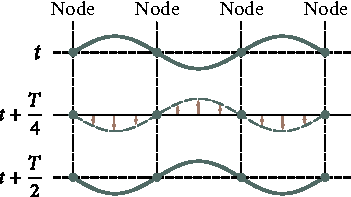
\includegraphics[scale=1]{figures/ch_14/fig_14_10.pdf}
% 		\caption[]{}
% 		\label{fig:14_10}
% 	\end{center}
% 	\vspace{-0.8cm}
% \end{figure}
\begin{figure}[!htb]
	\begin{minipage}[t]{0.48\linewidth}
		\begin{center}
			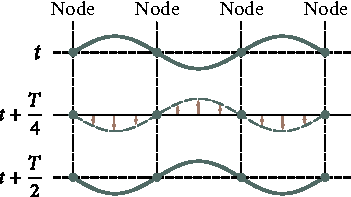
\includegraphics[scale=0.98]{figures/ch_14/fig_14_10.pdf}
			\caption[]{}
			\label{fig:14_10}
		\end{center}
	\end{minipage}
	\hfill{ }%space{-0.05cm}
	\begin{minipage}[t]{0.48\linewidth}
		\begin{center}
			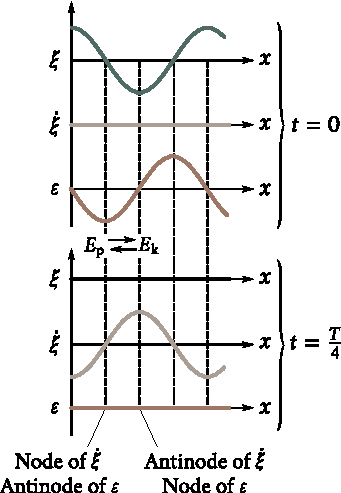
\includegraphics[scale=0.98]{figures/ch_14/fig_14_11.pdf}
			\caption[]{}
			\label{fig:14_11}
		\end{center}
	\end{minipage}
\vspace{-0.4cm}
\end{figure}

Đạo hàm \eqn{14_54} một lần theo $t$ và một lânf theo $x$, ta tìm được biểu thức vận tốc của phần tử $\dot{\xi}$ và sự biến dạng của môi trường $\varepsilon$:
\begin{align}
	\dot{\xi} &= \diff{\xi}{t} = - 2 \omega A \cos\parenthesis{ \frac{2\pi x}{\lambda} } \sin(\omega t), \label{eq:14_58}\\
	\varepsilon &= \diff{\xi}{x} = - 2 \frac{2\pi}{\lambda} A \sin\parenthesis{ \frac{2\pi x}{\lambda} } \cos(\omega t). \label{eq:14_59}
\end{align}

\noindent
Phương trình \eqref{eq:14_58} mô tả một sóng dừng của vận tốc và \eqn{14_59} mô tả độ biến dạng.

Hình \ref{fig:14_11} so sánh "các hình ảnh tức thời" của li độ, vận tốc, và độ biến dạng theo thời gian tại thời điểm $0$ và $T/4$. Các đồ thị cho thấy các nút sóng và bụng sóng của vận tốc trùng với li độ tương ứng; một cách tương tự, các nút sóng và bụng sóng của độ biến dạng cũng trùng với các nút sóng và bụng sóng của li độ. Khi $\xi$ và $\varepsilon$ tiến đến giá trị cực đại, $\dot{\xi}$ tiến đến không và ngược lại. Theo đó, nặng lượng của một sóng dừng được chuyến hóa hai lần trong một chu kỳ, một lần chuyển thành thế năng tập trung chủ yếu ở gần các nút sóng (nơi các bụng sóng biến dạng), và một lần chuyển hóa hoàn toàn thành động năng tập trung ở gần các bụng sóng (nơi mà vận tốc dao động mạnh nhất). Kết quả là năng lượng được tuyền qua lại giữa nút sóng và bụng sóng của nó. Trung bình mật độ năng thông truyền qua một mặt cắt bất kỳ của sóng bằng không.

\section{Dao động của dây}\label{sec:14_8}

Khi các dao động ngang được tạo ra trên một sợi dây căng được cố định hai đầu, các sóng dừng xuất hiện trên đó và các nút phải nằm ở các đầu dây. Vì vậy, chỉ có những dao động trên dây có độ dài bằng một số nguyên lần nửa bước sóng mới được tạo ra với cường độ đáng kể (\fig{14_12}). Điều này cho ta điều kiện
\begin{equation}\label{eq:14_60}
	l = n \frac{\lambda}{2}\quad \text{or}\quad \ab{\lambda}{n} = \frac{2l}{n}\quad (n = 1, 2, 3, \ldots)
\end{equation}

\noindent
($l$ là độ dài sợi dây). Các tần số theo đó ứng với bước sóng đã cho bởi \eqn{14_60}:
\begin{equation}\label{eq:14_61}
	\ab{\nu}{n} = \frac{v}{\ab{\lambda}{n}} = \frac{v}{2l} n \quad (n = 1, 2, 3, \ldots)
\end{equation}

\noindent
($v$ là vật tốc pha của sóng tính bởi lực căng dây và khối lượng trên mỗi đơn vị chiều dài dây, tức là mật độ khối dài của dây).

Các tần số $\ab{\nu}{n}$ được gọi là \textbf{các tần số tự nhiên} của dây. Các tần số tự nhiên bằng số nguyên lần tần số
\begin{equation*}
	\ab{\nu}{i} = \frac{v}{2l},
\end{equation*}

\noindent
gọi là \textbf{tần số cơ bản}.

\begin{figure}[!htb]
	\begin{center}
		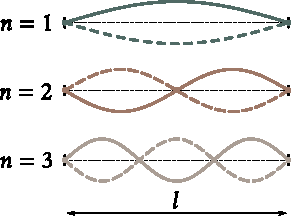
\includegraphics[scale=1]{figures/ch_14/fig_14_12.pdf}
		\caption[]{}
		\label{fig:14_12}
	\end{center}
	\vspace{-0.8cm}
\end{figure}

Các dao động điều hòa với tần số tuân theo \eqn{14_61} gọi là \textbf{tự nhiên} hay \textbf{các dao động chuẩn}. Chúng cũng được biết đến với cái tên \textbf{điều hòa}. Trong trường hợp tổng quát, dao động của một dây là chồng chập của các dao động điều hòa.

Các dao động của một sợi dây rất đặc biệt ở chỗ, theo các quan niệm cổ điển, chúng ta nhận được các giá trị rời rạc của một trong các đại lượng đặc trưng cho các dao động (tần số của chúng). Bản chất rời rạc như vậy là một ngoại lệ đối với vật lý cổ điển. Đối với các quá trình lượng tử, đó lại là quy luật chứ không phải ngoại lệ.

\section{Sóng âm}\label{sec:14_9}

Nếu sóng đàn hồi truyền trong không khí với tần số khoảng từ $\SI{16}{Hz}$ đến $\SI{20000}{Hz}$ đến tai người, chúng tạo ra âm thanh có thể nghe thấy được. Theo đó, sóng đàn hồi trong bất cứ môi trường nào có tần số nằm trong giới hạn trên được gọi là \textbf{sóng âm} hay đơn giản là \textbf{âm}. Sóng đàn hồi với tần số thấp hơn $\SI{16}{Hz}$ được gọi là \textbf{hạ âm}, và các tần số lớn hơn $\SI{20000}{Hz}$ được gọi là\textbf{siêu âm}. Tai người không thể nghe được hạ âm và siêu âm. 

Ta phân biệt các âm thanh nghe được thông qua \textbf{cao độ}, \textbf{âm sắc}, \textbf{chất lượng âm} và \textbf{cường độ}. Các đặc tính vật lý của một sóng ấm Mỗi đặc tính vật lý nhất định của sóng tương ứng với một đánh giá chủ quan.

Mỗi sóng âm thực tế không phải một dao động điều hòa đơn giản mà là chồng chập của các dao động điều hòa với tần số khác nhau. Tổng hợp các tần số của các dao động đại diện cho sóng âm được gọi là \textbf{âm phổ}. Nếu một sóng chứa các dao động với tất cả các tần số từ $\nu'$ đến $\nu''$, phổ của nó được gọi là \textbf{liên tục}. Nếu một sóng chứa các dao động với từng tần số $\nu_1$, $\nu_2$, $\nu_3$,... thì phổ được gọi là \textbf{rời rạc}. Các tiếng ồn có một âm phổ liên tục. Các dao dộng với một phổ với âm phổ vạch tạo ra cảm giác âm với nhiều hoặc ít hơn một cao độ xác định. một sóng âm như vậy được gọi là một \textbf{sóng tone} hay đơn giản là \textbf{tone}.

Cao độ của một tone xác định tần số cơ sở (nhỏ nhất) của nó. Cường độ tương đối của \textbf{bồi âm} (tức là của các dao động có các tần số $\nu_2$, $\nu_3$,...) xác định âm sắc, hay chất lượng âm của âm thanh. Sự khác biệt về phổ thành phần của các âm thanh tạo bởi các nhạc cụ giúp ta có thể phân biệt được bằng tai, ví dụ như một chiếc violin hay một chiếc piano.

Bởi cường độ của một sóng âm là giá trị trung bình theo thời gian của mật độ năng thông mang theo bởi một sóng âm. Để có thể nghe được, một sóng cần có một cường độ tối thiểu xác định được gọi là \textbf{ngưỡng nghe}. Tùy vào từng người, ngưỡng nghe có thể khác nhau và nó cũng phụ thuộc rất nhiều vào tần số của âm thanh đó. Tai người chủ yếu cảm nhận được các tần số trong khoảng từ $\SI{1000}{Hz}$ đến $\SI{4000}{Hz}$. Trong vùng tần số này, ngưỡng nghe trung bình sẽ vào khoảng \SI{e-12}{\watt\per\metre\squared}. Còn trong các tần số khác, nó sẽ cao hơn (xem đồ thị ở hình \fig{14_13}).

\begin{figure}[!htb]
	\begin{center}
		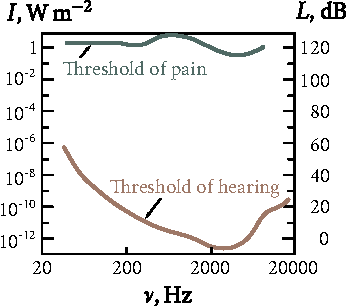
\includegraphics[scale=1]{figures/ch_14/fig_14_13.pdf}
		\caption[]{}
		\label{fig:14_13}
	\end{center}
	\vspace{-0.8cm}
\end{figure}

Ở cường độ vào khoảng $\SI{1}{W m^{-2}}$ đến  $\SI{10}{W m^{-2}}$, một sóng sẽ không còn được cảm nhận như một âm thanh và chỉ tạo ra cảm giác đau và áp lực vào tai. Giá trị của cường độ âm để xảy ra hiện tượng này được gọi là \textbf{ngưỡng đau}. Cũng giống như ngưỡng nghe, ngưỡng đau phụ thuộc vào tần số (xem đồ thị \fig{14_13}; đường cong trong hình vẽ là trung bình thính giác của một người bình thường). %trung bình thính giác của một người trong môi trường sống tự nhiên của họ.

Cường độ âm thanh chủ quan của một âm tăng chậm hơn cường độ sóng âm. Khi cường độ sóng âm tăng trong theo cấp số nhân, cường độ âm ta cảm nhận được thanh tăng theo cấp số cộng, hay tức là tăng tuyến tính. Trên cơ sở đó, \textbf{mức cường độ âm thanh} $L$ được tính bằng hàm logarit của tỷ số cường độ âm $I$ và cường độ $I_0$ lấy tại một điểm ban đầu:
\begin{equation}\label{eq:14_62}
	L = \log\parenthesis{\frac{I}{I_0}}.
\end{equation}

\noindent
Cường độ đầu $I_0$ bằng khoảng \SI{e-12}{\watt\per\metre\squared} nên ngưỡng nghe ở tần số \SI{1000}{\hertz} tại mức không ($L = 0$).

Đơn vị của mức cường độ âm thanh $L$ được tính bởi \eqn{14_62} được gọi là \text{bell} (B). Thông thường, \textbf{decibel} (dB), đơn vị nhỏ hơn bell mười lần, hay được sử dụng hơn. Giá trị của $L$ tính theo decibels bởi biểu thức
\begin{equation}\label{eq:14_63}
	L = 10 \log\parenthesis{\frac{I}{I_0}}.
\end{equation}

Tỷ số của hai cường độ $I_1$ và $I_2$ có thể được biểu diễn theo decibels: 
\begin{equation}\label{eq:14_64}
	L_{12} = 10 \log\parenthesis{\frac{I_1}{I_2}}.
\end{equation}

\noindent
Phương trình này có thể được sử dụng để mô tả sự giảm của cường độ (sự suy hao) của một sóng theo decibels.  Theo đó, ví dụ, một sự suy hao của \SI{20}{\decibel} cho thấy cường độ âm mất đi một trăm lần so với giá trị bay đầu.

Toàn bộ các cường độ mà một sóng tạo ra cảm giác âm cho tai người (từ \SI{e-12}{\watt\per\metre\squared}) có giá trị mức cường độ âm thanh $\SI{0}{dB}$ đến $\SI{130}{dB}$. Bảng \ref{table:14_1} cho ta giá trị gần đúng của mức âm cho các âm thanh được chọn.

Năng lượng mà sóng âm mang theo là cực kỳ nhỏ. Nếu ta giả thiết, ví dụ một cốc nước thủy tinh hấp thụ hoàn toàn năng lượng của một sóng âm có mức cường độ âm thanh \SI{70}{\decibel} (trong trường hợp này toàn bộ năng lượng bị hấp thụ mỗi giây là \SI{2e-7}{\watt}), theo đó, để làm nóng nước từ nhiệt độ phòng đến khi nó sôi sẽ mất cả hàng nghìn năm.

\begin{table}[!b]
	\renewcommand{\arraystretch}{1.2}
	\caption{}
	\vspace{-0.6cm}
	\label{table:14_1}
	\begin{center}\resizebox{0.65\linewidth}{!}{
			\begin{tabular}{lc}
				\toprule[1pt]
				\textbf{Âm thanh} & \textbf{Mức cường độ âm thanh}, \si{\decibel}\\
				\midrule[0.5pt]\midrule[0.5pt]
				Tiếng tik tak của một đồng hồ & $20$\\
				Thì thầm ở khoảng cách \SI{1}{\metre} & $30$\\
				Cuộc trò chuyện im lặng & $40$\\
				Lời nói với âm lượng vừa phải & $60$\\
				Tiếng nói chuyện ồn ào & $70$\\
				Shout & $80$\\
				Tiếng ồn của động cơ máy bay: &\\
				$\quad$ tại một khoảng cách \SI{5}{\metre} & $120$\\
				$\quad$ tại một khoảng cách \SI{3}{\metre} & $130$\\
				\bottomrule[1pt]
			\end{tabular}
	}\end{center}
\end{table}

Sóng siêu âm có thể được tạo ra dưới dạng chùm tia định hướng giống như chùm ánh sáng. Chùm siêu âm định hướng đã được ứng dụng rộng rãi để định vị các vật thể và xác định khoảng cách tới chúng trong nước. Người đầu tiên đưa ra ý tưởng về vị trí siêu âm là nhà vật lý lỗi lạc người Pháp Paul Langevin. Ông đã thực hiện ý tưởng này trong Thế chiến thứ nhất để phát hiện tàu ngầm.

Hiện tại, thiết bị định vị siêu âm được sử dụng để phát hiện các tảng băng trôi, bãi cá và những thứ tương tự.

Việc phát ra các âm thanh và đo lường thời gian âm thanh vọng lại, hay phản xạ từ núi, rừng, mặt nước của giếng,... để xác định khoảng cách bởi tích nữa thời gian này và vận tốc truyền sóng ấmấm đã được biết đến rộng rãi. Nguyên tắc này làm cơ sở cho thiết bị định vị (sonar) đã đề cập ở trên, cũng như thiết bị đo tiếng vang siêu âm được sử dụng để đo độ sâu và xác định độ nổi của đáy biển.

Định vị siêu âm cho phép những con dơi định hướng rất tốt khi bay trong bóng tối. Một con dơi sẽ đều đặn phát ra các xung của một tần số siêu âm và theo tín hiệu phản xạ mà tai nó nhận được, nó đánh giá khoảng cách đến các vật thể xung quanh với độ chính xác cao.

\section{Vận tốc sóng âm trong không khí}\label{sec:14_10}

Một sóng âm trong không khí là một chuỗi các sự nén giãn của không khí lan truyền trong không gian.
Thật vậy, áp suất tại mọi điểm trong không gian biến thiên $\Delta{p}$ theo chu kỳ quanh giá trị trung bình $p$ khi bỏ qua sóng trong không khí.
Do đó, giá trị liên tục của áp suất tại một điểm trong không gian có thể viết dưới dạng
\begin{equation*}
	p' = p + \Delta{p}.
\end{equation*}

Giả sử rằng sóng truyền dọc theo trục $x$.
Ta xét thể tích khí trong một hình trụ có diện tích đáy $S$ và chiều cao $\Delta{x}$ (\fig{14_14}), tương tự \sect{14_5} khi ta tìm vận tốc của sóng đàn hồi trong chất rắn.
Khối lượng của không khí trong thể tích hình trụ này là $\rho S\Delta{x}$, với $\rho$ là khối lượng riêng của không khí chưa bị dao động bởi sóng.
Chọn độ chia $\Delta{x}$ nhỏ nhất có thể ,các hình chiếu của gia tốc trên trục $x$ của các điểm trong hình trụ có thể xem như đồng nhất và bằng $\diffnpartialin{\xi}{t}2$.

\begin{figure}[!htb]
	\begin{center}
		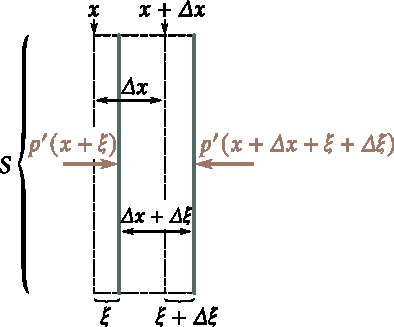
\includegraphics[scale=1]{figures/ch_14/fig_14_14.pdf}
		\caption[]{}
		\label{fig:14_14}
	\end{center}
	\vspace{-0.8cm}
\end{figure}

Để tìm hình chiếu dọc theo trục $x$ của lực tác dụng lên từng hình trụ nói trên, ta cần lấy tích của diện tích đáy trụ $S$ và chênh lệch áp suất giữa hai mặt cắt $(x+\xi)$ và $(x + \Delta{x} + \xi + \Delta{\xi})$. Làm lại các bước của \eqn{14_34}, ta được
\begin{equation*}
	F_x = - \diffpartial{p'}{x} S \Delta{x}
\end{equation*}

\noindent
[ta nhắc lại với độc giả rằng khi đạo hàm \eqn{14_34} ta đã giả thiết gần đúng $\Delta{\xi}\ll\Delta{x}$].

Thật vậy, ta đã tìm được khối lượng của một phần hình trụ không khí, gia tốc và lực tác dụng lên nó. Giờ ta viết định luật II Newton cho thể tích khí này:
\begin{equation*}
	(\rho S \Delta{x}) \diffnpartial{\xi}{t}{2} = - \diffpartial{p'}{x} S \Delta{x}.
\end{equation*}

\noindent
Sau khi triệt tiêu $S\Delta{x}$, ta có
\begin{equation}\label{eq:14_65}
	\rho \diffnpartial{\xi}{t}{2} = - \diffpartial{p'}{x}.
\end{equation}

Phương trình vi phân ta có hai ẩn đó là $\xi$ và $p'$.
Giờ ta sẽ cần biểu diễn một ẩn trong đó theo ẩn còn lại.
Để làm điều này, chúng ta sẽ tìm mối liên hệ giữa áp suất của khí và độ biến thiên tương đối trong thể tích của nó $\diffpartialin{\xi}{x}$.
Mối quan hệ này phụ thuộc vào bản chất tự nhiên của quá trình nén (hoặc giãn) của không khí.
Sự nén và giãn của không khí trong một sóng âm đều đặn đủ để  xem mối phân tử của môi trường đều không trao đổi nhiệt và quá trình này có thể xem như đoạn nhiệt. Trong một quá trình đoạn nhiệt, áp suất và thể tích của một khối lượng khí cho trước được mô tả bởi phương trình
\begin{equation}\label{eq:14_66}
	p V^{\gamma} = \text{constant},
\end{equation}

\noindent
với $\gamma$ là tỷ số của nhiệt dung khí đẳng áp và nhiệt dung khí đẳng tích [Xem Phương trình (10.42) của tập I].

Đưa vào \eqn{14_66}:
\begin{equation*}
	p (S \Delta{x})^{\gamma} = p'[S(\Delta{x}+\Delta{\xi})]^{\gamma} = p' \bracket{ S \parenthesis{\Delta{x} + \diffpartial{\xi}{x} \Delta{x}} }^{\gamma} = p' (S \Delta{x})^{\gamma} \parenthesis{1+ \diffpartial{\xi}{x}}^{\gamma}.
\end{equation*}

\noindent
Triệt tiêu $(S \Delta{x})^{\gamma}$ đi:
\begin{equation*}
	p = p' \parenthesis{1+ \diffpartial{\xi}{x}}^{\gamma}.
\end{equation*}

\noindent
Lấy gần đúng $\diffpartialin{\xi}{x}\ll 1$, ta khai triển $\parenthesis{1+ \diffpartialin{\xi}{x}}^{\gamma}$ thành dãy lũy thừa $\diffpartialin{\xi}{x}$ và bỏ qua các thành phần bậc cao của số hạng nhỏ.
Kết quả là
\begin{equation*}
	p = p' \parenthesis{ 1 + \gamma \diffpartial{\xi}{x} }.
\end{equation*}

\noindent
Ta giải phương trình này theo $p'$"
\begin{equation}\label{eq:14_67}
	p' = \frac{p}{\parenthesis{1 + \gamma \diffpartial{\xi}{x}}} \approx p \parenthesis{ 1 - \gamma \diffpartial{\xi}{x} }
\end{equation}

\noindent
[Ta sử dụng biểu thức $1/(1+x)\approx 1-x$ khi $x\ll 1$].
Nó sẽ là một vấn đề đơn giản để biểu diễn $\Delta{p}$ từ liên hệ ta đã tìm được:
\begin{equation}\label{eq:14_68}
	\Delta{p} = p' - p = - \gamma p \diffpartial{\xi}{x}.
\end{equation}

Vì độ lớn của $\gamma$ gần với một đơn vị, dựa vào \eqn{14_68} nên $|\diffpartialin{\xi}{x}| \approx |\Delta{p}/p|$.
Do đó, điều kiện $\diffpartialin{\xi}{x}\ll 1$ cho biết rằng độ lệch của áp suất so với giá trị trung bình rất nhỏ so với áp suất của nó.
Điều này hoàn toàn đúng: với âm to nhất, biên độ của dao các dao động của áp suất không khí không đến \SI{1}{\mmHg}, trong khi áp suất khí quyển $p$ có độ lớn \SI{e3}{\mmHg}.

Đạo hàm \eqn{14_67} theo riêng phần $x$, ta tìm được
\begin{equation*}
	\diffpartial{p'}{x} = - \gamma p \diffnpartial{\xi}{x}{2}.
\end{equation*}

\noindent
Cuối cùng, sử dụng giá trị của $\diffpartialin{p'}{x}$ trong \eqn{14_65}, ta có được phương trình vi phân
\begin{equation*}
	\diffnpartial{\xi}{x}{2} = \frac{\rho}{\gamma p} \diffnpartial{\xi}{t}{2}.
\end{equation*}

\noindent
So sánh nó với phương trình sóng \eqref{eq:14_29}, ta có thể biểu diễn vận tốc của sóng âm trong không khí:
\begin{equation}\label{eq:14_69}
	v = \parenthesis{\gamma \frac{p}{\rho}}^{1/2}
\end{equation}

\noindent
(ta nhắc lại với độc giả rằng $p$ và $\rho$ là áp suất và khối lượng riêng của không khí khi chưa dao động bởi sóng)

Ở áp suất khí quyển và nhiệt độ phòng, hầu hết các khí sẽ có tính chất gần giống như khí lý tưởng.
Vì vậy, ta có thể giả thiết rằng tỷ số $p/\rho$ bằng $RT/M$, với $R$ là hằng số khí lý tưởng, $T$ là nhiệt độ tuyệt đối, và $M$ là khối lượng mol của một loại khí [xem Phương trình (10.22) của Tập 1].
Thay giá trị này vào \eqn{14_69}, ta có biểu thức vận tốc sóng âm trong không khí:
\begin{equation}\label{eq:14_70}
	v = \parenthesis{ \frac{\gamma RT}{M}}^{1/2}.
\end{equation}

\noindent
Phương trình này cho thấy vận tốc âm tỷ lệ với căn bậc hai của nhiệt độ và không phụ thuộc vào áp suất.

Vận tốc nhiệt trung bình của không khí được tính bởi biểu thức
\begin{equation*}
	\average{\ab{v}{mol}} = \parenthesis{\frac{8RT}{\pi M}}^{1/2}
\end{equation*}

\noindent
[xem Phương trình (11.70) của Tập I].
So sánh phương trình này với \eqn{14_70} cho thấy vận tốc sóng âm trong không khí liên hệ với vận tốc nhiệt trung bình qua biểu thức
\begin{equation}\label{eq:14_71}
	v = \average{\ab{v}{mol}} \parenthesis{\frac{\gamma\pi}{8}}^{1/2}.
\end{equation}

\noindent
Thay giá trị của $\gamma$ cho không khí là $1.4$ dẫn tới biểu thức $v\approx 3\average{\ab{v}{mol}}/4$.
Giá trị cực đại của $\gamma$ là $5/3$.
Trong trường hợp này, $v\approx 4\average{\ab{v}{mol}}/5$.
Vì vậy, vận tốc sóng âm có cùng cỡ độ lớn với trung bình vận tốc nhiệt của không khí, nhưng nó luôn thấp hơn $\average{\ab{v}{mol}}$.

Hãy tính giá trị của vận tốc sóng trong không khí tại nhiệt độ \SI{290}{\kelvin} (nhiệt độ phòng).
Với không khí, ta có $\gamma=1.40$, $M=\SI{29e-3}{\kilo\gram\per\mole}$.
Hằng số khí lý tưởng là $R=\SI{8.31}{\joule\per\mole\per\kelvin}$.
Thay các giá trị này vào \eqn{14_70}, ta có
\begin{equation*}
	v = \parenthesis{\frac{\gamma RT}{M}}^{1/2} = \parenthesis{\frac{1.4\times 8.31 \times 290}{\num{29e-3}}}^{1/2} = \SI{340}{\metre\per\second}.
\end{equation*}

\noindent
Giá trị của vận tốc sóng âm trong không khí mà ta đã tìm rất khớp với giá trị ta tìm được bằng thực nghiệm.

Ta sẽ tìm quan hệ giữa cường độ của một sóng âm $I$ và biên độ của áp suất dao động $\ab{(\Delta{p})}{m}$.
Ta đã đề cập trong \sect{14_9} rằng bởi cường độ của sóng là giá trị trung bình của mật độ năng thông.
Vì vậy,
\begin{equation}\label{eq:14_72}
	I = \frac{1}{2} \rho A^2 \omega^2 v
\end{equation}

\noindent
[xem \eqn{14_48}].
Ở đây, $p$ là mật độ không khí khi không dao động, $A$ là biên độ dao động của các phần tử của môi trường, tức là biên độ của các dao động trong li độ $\xi$, $\omega$ là tần số, và $v$ là vận tốc pha của sóng.
Ta phải ghi chú rằng trong trường hợp này các phần từ của môi trường được hiểu là thể tích vĩ mô (tức là trong một số lượng lớn không khí), và không phải các phân tử; kích thước tuyến tính của các phần thể tích này rất nhỏ so với bước sóng.

Giả sử rằng $\xi$ biến thiên theo quy luật
$\xi=A\cos(\omega t-kx+\alpha)$.
Như vậyvậy,
\begin{equation*}
	\diffpartial{\xi}{x} = Ak \sin(\omega t - k x + \alpha) = A \frac{\omega}{v} \sin(\omega t - k x + \alpha).
\end{equation*}

\noindent
Thay giá trị này vào \eqn{14_68}, ta thấy
\begin{equation*}
	\Delta{p} = - \gamma p A \frac{\omega}{v} \sin(\omega t - kx + \alpha) = - \ab{(\Delta{p})}{m} \sin(\omega t - kx + \alpha),
\end{equation*}

\noindent
Với
\begin{equation}\label{eq:14_73}
	A = \frac{\ab{(\Delta{p})}{m} v^2}{\gamma p \omega}.
\end{equation}

\noindent
Dùng cách biểu diễn trong \eqn{14_72}, ta có
\begin{equation*}
	I = \frac{1}{2} \rho \frac{\ab{(\Delta{p})^2}{m} v^2}{\gamma^2 p^2 \omega^2} \omega^2 v = \frac{\ab{(\Delta{p})^2}{m}}{2 \gamma^2 \rho v} \parenthesis{\frac{\rho}{p}}^2 v^4.
\end{equation*}

\noindent
Tính đến việc $v^4 = (\gamma RT/M)^2$, và $(p/\rho)^2 = (RT/M)^2$ [xem \eqn{14_70} và lời dẫn trước đó], ta có thể viết rằng
\begin{equation}\label{eq:14_74}
	I = \frac{\ab{(\Delta{p})^2}{m}}{2 \rho v}.
\end{equation}

\noindent
Ta có thể dùng phương trình này để tính toán gần đúng giá trị biên độ của các dao động áp suất không khí trong khoản tiếng ồn từ \SI{0}{\decibel} đến \SI{130}{\decibel}.
Giá trị này vào khoảng \SI{3e-5}{\pascal} (\SI{2e-7}{\mmHg}) đến \SI{100}{\pascal} (khoảng \SI{1}{\mmHg}).

Giờ ta sẽ đánh giá biên độ dao động của của các phần tử $A$ và vận tốc của các phần tử $\ab{(\dot{\xi})}{m}$.
Ta sẽ bắt đầu với một đánh giá của đại lượng $A$ tính bởi \eqn{14_73}.
Thay vào $v/\omega=\lambda/(2\pi)$, ta có được biểu diễn
\begin{equation}\label{eq:14_75}
	\frac{A}{\lambda} = \frac{1}{2\pi\gamma} \frac{\ab{(\Delta{p})^2}{m}}{p} \approx 0.1 \frac{\ab{(\Delta{p})^2}{m}}{p}
\end{equation}

\noindent
($\gamma \approx 1.5$, do đó, $2 \pi \gamma \approx 10$).
Ở âm thanh \SI{130}{\decibel}, tỷ số $\ab{(\Delta{p})^2}{m}/p$ có giá trị vào khoảng \num{e-3}, trong khi ở âm thanh \SI{60}{\decibel} tỷ số này là \num{2e-7}.
Độ dài của các sóng âm trong không khí vào khoảng \SI{21}{\metre} (ở tần số $\nu = \SI{16}{\hertz}$) tới \SI{17}{\milli\metre} (ở tần số $\nu = \SI{20000}{\hertz}$).
Đưa các giá trị trên vào \eqn{14_75}, ta tìm được tại âm thanh \SI{60}{\decibel} biên độ dao động của các phần tử vào khoảng \SI{4e-4}{\milli\metre} cho sóng dài nhất và \SI{3e-7}{\milli\metre} cho sóng ngắn nhất.
Tại một âm thanh \SI{130}{\decibel}, biên độ các dao động cho các sóng dài nhất vào khoảng \SI{2}{\milli\metre}.

Cho các dao động điều hòa, biên độ của vận tốc $\ab{(\dot{\xi})}{m}$ bằng ly độ $A$ nhân với tần số $\omega$: $\ab{(\dot{\xi})}{m} = A\omega$.
Nhân \eqn{14_75} với $\omega$, ta có
\begin{equation}\label{eq:14_76}
	\frac{\ab{(\dot{\xi})}{m}}{v} = \frac{1}{\gamma} \frac{\ab{(\Delta{p})}{m}}{p} \approx \frac{\ab{(\Delta{p})}{m}}{p}.
\end{equation}

\noindent
Theo đó, tại một âm thanh \SI{130}{\decibel}, biên độ vận tốc sẽ vào khoảng $\SI{340}{\metre\per\second}\times\num{e-3}=\SI{0.34}{\metre\per\second}$.
Tại một âm thanh \SI{60}{\decibel}, biên độ của vận tốc sẽ là \SI{0.1}{\milli\metre\per\second}.
Ta cần ghi chú rằng không giống như biên độ của li độ, biên độ của vận tốc không phụ thuộc vào bước sóng.

\section{Hiệu ứng Doppler cho sóng âm}\label{sec:14_11}

Giả sử có một thiết bị đo các dao động của môi trường gọi là máy thu đặt trong chất lỏng cách nguồn sóng một khoảng nhất định.
Nếu nguồn và máy thu sóng đứng yên so với môi trường truyền sóng, tần số của các dao động sẽ được ghi nhận ở máy thu sẽ bằng tần số $\nu$ của các dao động phát ra từ nguồn.
Nếu cả nguồn hoặc máy thu hoặc cả hai đều chuyển động tương đối so với môi trường truyền sóng, tần số $\nu$ thu được bởi máy thu có thể khác với tần số $\nu_0$.
Hiện tượng này được gọi là \textbf{hiệu ứng Doppler}. [Nó được đặt tên theo nhà khoa học người Úc Christian Doppler (1803-1853), người đã mô tả lại hiệu ứng này đối với sóng ánh sáng.]

Ta giả thiết rằng nguồn và máy thu chuyển động dọc theo một đường thẳng đi qua chúng.
Ta sẽ giả thiết vận tốc của nguồn là $\ab{v}{s}$ hướng theo chiều dương nếu nó chuyển động tiến về phía máy thu và âm nếu nó chuyển động ra xa máy thu.
Tương tự, ta cũng giả thiết vận tốc của máy thu là $\ab{v}{r}$ dương nếu nó chuyển động về phía nguồn và âm nếu nó chuyển động ra xa khỏi nguồn.

Nếu nguồn đứng yên và dao động với tần số $\nu_0$, tại thời điểm mà nguồn hoàn thành $\nu_0$ lần dao động, đỉnh của sóng tạo bởi dao động đầu tiên sẽ đi được một đoạn $v$ trong môi trường truyền sóng ($v$ là vận tốc lan truyền tương đối của sóng với môi trường).
Cho nên, có $\nu_0$ đỉnh và đáy của sóng tạo bởi nguồn trong một giây sẽ được bao bởi độ dài $v$.
Nếu nguồn chuyển động tương đối so với môi trường bằng một vận tốc $\ab{v}{s}$, tại thời điểm nguồn hoàn thành dao động thứ $\nu_0$, đỉnh tạo bởi dao động đầu tiện sẽ đi được một đoạn $v-\ab{v}{s}$ từ nguồn (\fig{14_15}).
Vì thế, độ dài $v-\ab{v}{s}$ sẽ chứa $\nu_0$ đỉnh và đáy của một sóng, cho nên bước sóng sẽ thành
\begin{equation}\label{eq:14_77}
	\lambda = \frac{v - \ab{v}{s}}{\nu_0}.
\end{equation}

\begin{figure}[!htb]
	\begin{center}
		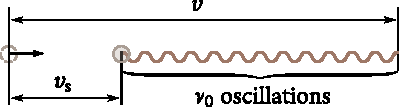
\includegraphics[scale=1]{figures/ch_14/fig_14_15.pdf}
		\caption[]{}
		\label{fig:14_15}
	\end{center}
	\vspace{-0.8cm}
\end{figure}

Mỗi giây, các đỉnh và đáy trong đoạn chiều dài $v$ sẽ đi qua máy thu đứng yên.
Nếu máy thu chuyển động với vận tốc $\ab{v}{r}$, tại lúc kết thúc thời gian một giây, máy thu này sẽ ghi nhận các đáy trong đoạn khoảng cách $v$ tính từ vị trí hiện tại của nó.
Từ đó, trong một giây, máy thu sẽ ghi nhận các dao độngpharn hồi qua các đỉnh và đáy nằm trong khoảng độ dài $v+\ab{v}{r}$ (\fig{14_16}) và tần số dao động đó là
\begin{equation*}
	\nu = \frac{v + \ab{v}{r}}{\lambda}.
\end{equation*}

\noindent
Thay $\lambda$ từ \eqn{14_77}, ta có
\begin{equation}\label{eq:14_78}
	\nu = \nu_0 \parenthesis{\frac{v + \ab{v}{r}}{v - \ab{v}{s}}}.
\end{equation}
Dựa vào \eqn{14_78}, việc máy thu và nguồn tiến lại gần nhau và làm giảm khoảng cách giữa chúng sẽ khiến cho tần số $\nu$ mà máy thu ghi nhận được lớn hơn tần số $\nu_0$ của nguồn.
Nếu khoảng cách giữa nguồn và máy thu tăng lên, tần số $\nu$ sẽ nhỏ hơn $\nu_0$.

\begin{figure}[!htb]
	\begin{center}
		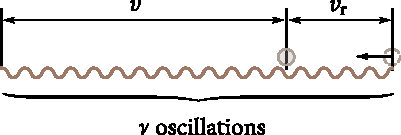
\includegraphics[scale=1]{figures/ch_14/fig_14_16.pdf}
		\caption[]{}
		\label{fig:14_16}
	\end{center}
	\vspace{-0.8cm}
\end{figure}

Nếu như hướng của các vận tốc $\ab{\vec{v}}{s}$ và $\ab{\vec{v}}{r}$ trùng với đường thẳng đi qua nguồn và máy thu, các hình chiếu của các vector $\ab{\vec{v}}{s}$ và $\ab{\vec{v}}{r}$ lên đường thẳng nối giữa nguồn và máy phát sẽ phải thay cho $\ab{v}{s}$ và $\ab{v}{s}$ trong \eqn{14_78}.

Xem xét \eqn{14_78} cho thấy hiệu ứng Doppler cho các sóng âm được tính bởi vận tốc tương đối của nguồn và máy thu so với môi trường truyền sóng.
Hiệu ứng Doppler cũng được quan sát với các sóng ánh sáng, nhưng phương trình sẽ có một chút sự khác biệt so với \eqn{14_78}.
Điều này cho thấy không có một môi trường nào tồn tại cho sóng ánh sáng.
Vì thế, các vận tốc tương đối nguồn và máy thu của ánh sáng so với môi trường là vô nghĩa.
Đối với ánh sáng, ta có thể nói rằng chỉ có vận tốc tương đối giữa nguồn và máy thu.
Hiệu ứng Doppler cho ánh sáng phụ thuộc vào độ lớn và hướng của vận tốc này.
Hiệu ứng này sẽ được khảo sát với sóng ánh sách ở \sect{21_4}.
